基于”Proposal + Classification”的Object Detection的方法,RCNN系列(R-CNN、SPPnet、Fast R-CNN以及Faster R-CNN)取得了非常好的效果,因为这一类方法先预先回归一次边框,然后再进行骨干网络训练,所以精度要高,这类方法被称为two stage的方法。但也正是由于此,这类方法在速度方面还有待改进。由此,YOLO[8]应运而生,YOLO系列只做了一次边框回归和打分,所以相比于RCNN系列被称为one stage的方法,这类方法的最大特点就是速度快。但是YOLO虽然能达到实时的效果,但是由于只做了一次边框回归并打分,这类方法导致了小目标训练非常不充分,对于小目标的检测效果非常的差。简而言之,YOLO系列对于目标的尺度比较敏感,而且对于尺度变化较大的物体泛化能力比较差。

针对YOLO和Faster R-CNN的各自不足与优势,WeiLiu等人提出了Single Shot MultiBox Detector,简称为SSD。SSD整个网络采取了one stage的思想,以此提高检测速度。并且网络中融入了Faster R-CNN中的anchors思想,并且做了特征分层提取并依次计算边框回归和分类操作,由此可以适应多种尺度目标的训练和检测任务。SSD的出现使得大家看到了实时高精度目标检测的可行性。

SSD和Yolo一样都是采用一个CNN网络来进行检测,但是却采用了多尺度的特征图,其基本架构如图3所示。下面将SSD核心设计理念总结为以下三点:

\textbf{1、采用多尺度特征图用于检测 }

所谓多尺度采用大小不同的特征图,CNN网络一般前面的特征图比较大,后面会逐渐采用stride=2的卷积或者pool来降低特征图大小,这正如图3所示,一个比较大的特征图和一个比较小的特征图,它们都用来做检测。这样做的好处是比较大的特征图来用来检测相对较小的目标,而小的特征图负责检测大目标,如图4所示,8x8的特征图可以划分更多的单元,但是其每个单元的先验框尺度比较小。
\begin{uscfigure}
	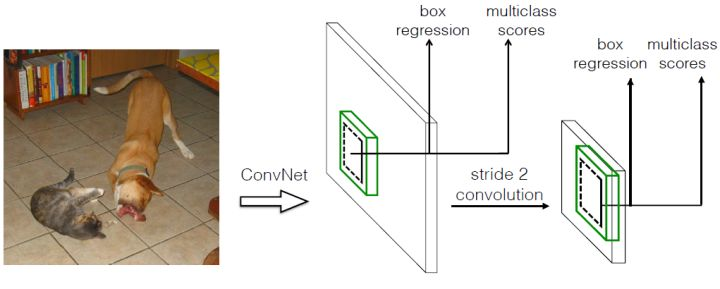
\includegraphics[width=\textwidth]{./Pictures/ssd_(1).jpg}	
	\caption{RCNN}
\end{uscfigure}
\textbf{2、采用卷积进行检测}

与Yolo最后采用全连接层不同,SSD直接采用卷积对不同的特征图来进行提取检测结果。对于形状为 $m\times n \times p $的特征图,只需要采用$ 3\times 3 \times p $这样比较小的卷积核得到检测值。 
\begin{uscfigure}
	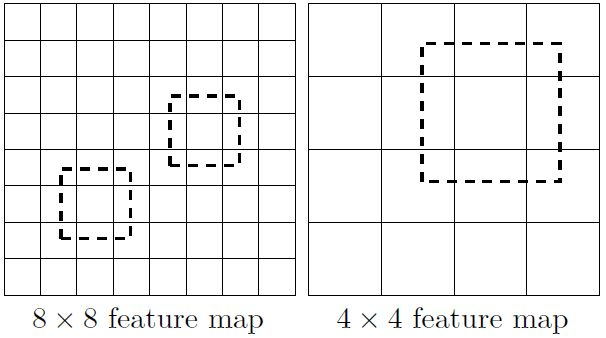
\includegraphics[width=\textwidth]{./Pictures/ssd_(2).jpg}	
	\caption{RCNN}
\end{uscfigure}
\textbf{3、设置先验框 }

在Yolo中,每个单元预测多个边界框,但是其都是相对这个单元本身(正方块),但是真实目标的形状是多变的,Yolo需要在训练过程中自适应目标的形状。而SSD借鉴了Faster R-CNN中anchor的理念,每个单元设置尺度或者长宽比不同的先验框,预测的边界框(bounding boxes)是以这些先验框为基准的,在一定程度上减少训练难度。一般情况下,每个单元会设置多个先验框,其尺度和长宽比存在差异,如图5所示,可以看到每个单元使用了4个不同的先验框,图片中猫和狗分别采用最适合它们形状的先验框来进行训练,后面会详细讲解训练过程中的先验框匹配原则。
\begin{uscfigure}
	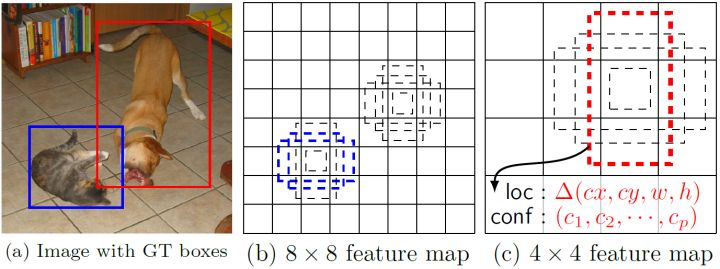
\includegraphics[width=\textwidth]{./Pictures/ssd_(3).jpg}	
	\caption{RCNN}
\end{uscfigure}